\documentclass[a4paper,12pt]{extarticle}
\usepackage[utf8x]{inputenc}
\usepackage[T1,T2A]{fontenc}
\usepackage[russian]{babel}
\usepackage{hyperref}
\usepackage{indentfirst}
\usepackage{listings}
\usepackage{color}
\usepackage{here}
\usepackage{array}
\usepackage{multirow}
\usepackage{graphicx}

\usepackage{caption}
\renewcommand{\lstlistingname}{Программа} % заголовок листингов кода

\bibliographystyle{ugost2008ls}

\usepackage{listings}
\lstset{ %
extendedchars=\true,
keepspaces=true,
language=C,						% choose the language of the code
basicstyle=\footnotesize,		% the size of the fonts that are used for the code
numbers=left,					% where to put the line-numbers
numberstyle=\footnotesize,		% the size of the fonts that are used for the line-numbers
stepnumber=1,					% the step between two line-numbers. If it is 1 each line will be numbered
numbersep=5pt,					% how far the line-numbers are from the code
backgroundcolor=\color{white},	% choose the background color. You must add \usepackage{color}
showspaces=false				% show spaces adding particular underscores
showstringspaces=false,			% underline spaces within strings
showtabs=false,					% show tabs within strings adding particular underscores
frame=single,           		% adds a frame around the code
tabsize=2,						% sets default tabsize to 2 spaces
captionpos=t,					% sets the caption-position to top
breaklines=true,				% sets automatic line breaking
breakatwhitespace=false,		% sets if automatic breaks should only happen at whitespace
escapeinside={\%*}{*)},			% if you want to add a comment within your code
postbreak=\raisebox{0ex}[0ex][0ex]{\ensuremath{\color{red}\hookrightarrow\space}},
texcl=true,
inputpath=listings,                     % директория с листингами
}

\usepackage[left=2cm,right=2cm,
top=2cm,bottom=2cm,bindingoffset=0cm]{geometry}

%% Нумерация картинок по секциям
\usepackage{chngcntr}
\counterwithin{figure}{section}
\counterwithin{table}{section}

%%Точки нумерации заголовков
\usepackage{titlesec}
\titlelabel{\thetitle.\quad}
\usepackage[dotinlabels]{titletoc}

%% Оформления подписи рисунка
\addto\captionsrussian{\renewcommand{\figurename}{Рисунок}}
\captionsetup[figure]{labelsep = period}

%% Подпись таблицы
\DeclareCaptionFormat{hfillstart}{\hfill#1#2#3\par}
\captionsetup[table]{format=hfillstart,labelsep=newline,justification=centering,skip=-10pt,textfont=bf}

%% Путь к каталогу с рисунками
\graphicspath{{fig/}}
 	% подключение настроек
\begin{document}	     % начало документа
\begin{titlepage}	% начало титульной страницы

	\begin{center}		% выравнивание по центру

		\large Санкт-Петербургский Политехнический Университет Петра Великого\\
		\large Институт компьютерных наук и технологий \\
		\large Кафедра компьютерных систем и программных технологий\\[6cm]
		% название института, затем отступ 6см
		
		\huge Сети и телекоммуникации\\[0.5cm] % название работы, затем отступ 0,5см
		\large Отчет по лабораторной работе\\[0.1cm]
		\large Программирование сокетов протоколов TCP\\[5cm]

	\end{center}


	\begin{flushright} % выравнивание по правому краю
		\begin{minipage}{0.25\textwidth} % врезка в половину ширины текста
			\begin{flushleft} % выровнять её содержимое по левому краю

				\large\textbf{Работу выполнил:}\\
				\large Волкова М.Д.\\
				\large {Группа:} 43501/3\\
				
				\large \textbf{Преподаватель:}\\
				\large Алексюк А.О.

			\end{flushleft}
		\end{minipage}
	\end{flushright}
	
	\vfill % заполнить всё доступное ниже пространство

	\begin{center}
	\large Санкт-Петербург\\
	\large \the\year % вывести дату
	\end{center} % закончить выравнивание по центру

\thispagestyle{empty} % не нумеровать страницу
\end{titlepage} % конец титульной страницы

\vfill % заполнить всё доступное ниже пространство
   % Титульная страница

\section{Цель работы}
Изучение принципов программирования сокетов протоколов TCP.

\section{Программа работы}
\begin{itemize}
\item разработать простейший клиент и сервер на основе протоколов TCP 
\item разработать прикладной протокол в соответствии с индивидуальным заданием, реализовать протокол в виде клиент-серверного приложения на основе протоколов TCP
\end{itemize}

\section{Ход выполнения работы}

\subsection{Простейшие клиент и сервер}
Простейшие клиент и сервер были выполнены на основе протоколов TCP, а также адаптированы под ОС Windows и Linux. Сервер выполняет функции эхо-сервера, т.е. принимает сообщения от клиентов и посылает копии обратно. Клиент посылает сообщение, после чего завершается.

\subsection{Индивидуальное задание}
Разработать приложение клиент и приложение сервер системы поиска/публикации новостей. Новости сгруппированы по темам. Каждая новость имеет уникальный идентификатор, название и текст новости.

Серверное приложение реализует следующие функции:
\begin{itemize}
\item Прослушивание определенного порта

\itemОбработка запросов по подключению

\item Поддержка одновременной работы нескольких клиентов системы

\item Прием запросов от клиента на передачу списка тем, списка новостей по теме, текста новости, добавление новости по теме

\item Осуществление добавления тем, новостей по темам

\item Передача списков тем, списков новостей и текстов новостей

\item Обработка запроса на отключение клиента

\item Принудительное отключение клиента
\end{itemize}

Клиентское приложение реализует следующие функции:

\begin{itemize}
\item Установление соединения с сервером

\item Передача запросов на передачу списка тем, списка новстей по теме, текста новости, добавление новости по теме

\item Получение результатов от сервера

\item Разрыв соединения

\item Обработка ситуации отключения клиента сервером
\end{itemize}


\subsubsection{Описание протокола}
Сообщение клиента  содержит команду, определяющее тип сообщения. 
\begin{itemize}
\item Команда для получения списка тем - 1
\item Команда для добавления новости - 2
\item Команда для выхода клиента - 3
\end{itemize}
В любом другом случае, появится сообщение об ошибке.\\

Сообщение сервера содержит команду, определяющее тип сообщения.
\begin{itemize}
\item Команда отключения клиента - kill
\item Просмотр подключенных клиентов  - online
\item Закрытие системы - shutdown
\end{itemize}


\subsubsection{Описание структуры приложения}
\paragraph{Сервер:}
\begin{itemize}
\item Создание сокета
\item Создание потока для прослушивания сокета
\item Чтеник команд от сервера
\item Чтеник команд от клиента
\item Получение сообщения от клиентов
\item Анализ сообщения
\item Ответ на сообщение
\end{itemize}

\paragraph{Клиент:}
\begin{itemize}
\item Чтение IP адреса сервера
\item Подключение к серверу
\item Создание потока
\item Чтение данных от сервера и реакция
\item Отправка команд серверу
\item Поток для получения данных от сервера
\end{itemize}


\section{Тестирование}

\begin{figure}[H]
	\begin{center}
		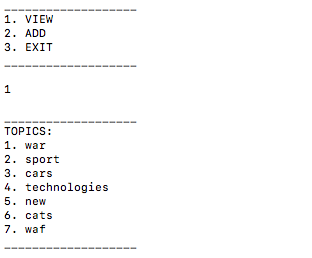
\includegraphics[scale=0.7]{1}
		\caption{Просмотр списка тем} 
		\label{pic:pic_name} % название для ссылок внутри кода
	\end{center}
\end{figure}

\begin{figure}[H]
	\begin{center}
		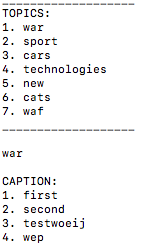
\includegraphics[scale=0.7]{2}
		\caption{Просмотр название новостей по теме war} 
		\label{pic:pic_name} % название для ссылок внутри кода
	\end{center}
\end{figure}

\begin{figure}[H]
	\begin{center}
		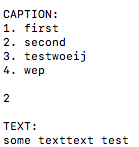
\includegraphics[scale=0.7]{3}
		\caption{Просмотр текста второй новости} 
		\label{pic:pic_name} % название для ссылок внутри кода
	\end{center}
\end{figure}

\begin{figure}[H]
	\begin{center}
		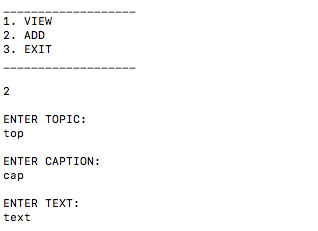
\includegraphics[scale=0.7]{4}
		\caption{Добавление новой новости} 
		\label{pic:pic_name} % название для ссылок внутри кода
	\end{center}
\end{figure}

\begin{figure}[H]
	\begin{center}
		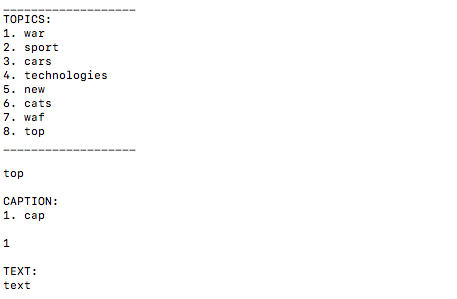
\includegraphics[scale=0.7]{5}
		\caption{Просмотр добавленной новости на втором клиенте} 
		\label{pic:pic_name} % название для ссылок внутри кода
	\end{center}
\end{figure}

\begin{figure}[H]
	\begin{center}
		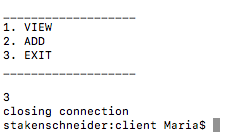
\includegraphics[scale=0.7]{6}
		\caption{Выход клиента} 
		\label{pic:pic_name} % название для ссылок внутри кода
	\end{center}
\end{figure}

\begin{figure}[H]
	\begin{center}
		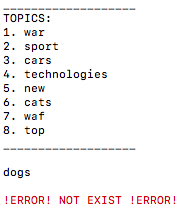
\includegraphics[scale=0.7]{7}
		\caption{Приемер вывода ошибки} 
		\label{pic:pic_name} % название для ссылок внутри кода
	\end{center}
\end{figure}


\section{Выводы}

В ходе работы были изучены принципы программирования сокетов с использованием протокола TCP.\\
Во время выполнения индивидуального задания была реализована клиент-серверная программа системы поиска/публикации новостей, с написанием собственного протокола на основе TCP. 
В результате этого были изучены принципы программирования сокетов TCP. Основной проблемой при реализации приложения на TCP была необходимость контроля длины посылки. Ее решением стало добавление символа окончания посылки. TCP требует установления соединения, поэтому на сервере выделяется поток, в котором происходит прием запросов на соединение от клиентов через выделенный для этого сокет. После подключения очередного клиента порождается отдельный поток, осуществляющий обмен пакетами с этим клиентом через отдельный сокет. 


\end{document}
